\documentclass[12pt]{article} 	% Type de document & taille de police
\usepackage[margin=2.53cm]{geometry}  % Marges normales de Word
\usepackage[french]{babel}  % Langue
\usepackage[utf8]{inputenc}  % Saisi du texte : permet les accents
\usepackage[T1]{fontenc} 	% Encodage du document
\setlength{\parindent}{0pt}  % Pas d'indentation
\setlength{\parskip}{1em}  % Passer une ligne après chaque paragraphe
\usepackage{hyperref}	% Inclure les liens
\usepackage{graphicx}	% Inclure des images
\topskip0pt  % Permet \vspace*{\fill} pour centrer verticalement
\usepackage{xcolor} % Texte coloré

\newcommand\capitalLetter[1]{\textsc{\MakeLowercase{#1}}}

%%%%%%%%%%%%%%%%%%%%% Section à remplir %%%%%%%%%%%%%%%%%%%%%
\newcommand\titreDuCours{Stage en génie logiciel III}
\newcommand\sigleCoursStage{GLO-2531}
\newcommand\session{Été 2042}
\newcommand\acronymeDuBac{GLO}

\newcommand\titreStagiaire{TitreDuStagiaire}
\newcommand\nomCompagnie{NomCompagnie}

\newcommand\dateRemise{42 avril 2042}
\newcommand\prenomStagiaire{Lesta}
\newcommand\nomStagiaire{Giaire}
\newcommand\idul{123 456 789}

\newcommand\prenomSuperviseur{Lesuper}
\newcommand\nomSuperviseur{Viseur}
\newcommand\titreSuperviseur{TitreDeMonsuperViseur}

% Changer si la page de présentation ne tient pas sur une page
\newcommand\distanceEnteteEtNomStage{4cm}
\newcommand\distanceTypeRapportEtDestinataire{5cm}
%%%%%%%%%%%%%%%%%%%%%%%%%%%%%%%%%%%%%%%%%%%%%%%%%%%%%%%%%%%%%

\begin{document}

\thispagestyle{empty}
\begin{minipage}[t]{8.5cm}
    \vspace{0pt}
    \begin{flushleft}
        \hspace{-1cm}
\includegraphics[width=5cm]{img/ulaval_logo.jpg}\\
        \hspace{-1cm}{\sf\scriptsize \textbf{\capitalLetter{faculté des sciences et génie}}}\\[-0.2cm]
    \end{flushleft}
\end{minipage}
\begin{minipage}[t]{8.5cm}
    \begin{flushright}
        \hspace*{2cm} \\
        \hspace*{1cm}\titreDuCours\\
        \hspace*{1cm}\sigleCoursStage\\
        \hspace*{1cm}\session\\
        \hspace*{1cm}Baccalauréat en {\acronymeDuBac}\\
    \end{flushright}
\end{minipage}

\vspace{\distanceEnteteEtNomStage}
\begin{center}
    \large {\titreStagiaire}  - {\nomCompagnie} \\
    \vspace{1cm}
    \large Rapport fin de stage \\

    \vspace{\distanceTypeRapportEtDestinataire}
    \fontsize{14.4}{14.4}\textbf {Destinataire}\\

    \vspace{0.5cm}
    \large Département des stages en milieu pratique \\

\end{center}
\vspace{3cm}
\begin{flushleft}
    Date de remise : {\dateRemise}
\end{flushleft}

\par\noindent\rule{\textwidth}{0.4pt}
\begin{minipage}[t]{6cm}
    \begin{flushleft}
        \textbf {\prenomStagiaire~\nomStagiaire}\\
        \idul
    \end{flushleft}
\end{minipage}
\begin{minipage}[t]{10cm}
    \begin{flushright}
        \hspace*{1cm}\textbf {\prenomSuperviseur~\nomSuperviseur~- \titreSuperviseur} \\
    \end{flushright}
\end{minipage}

\newpage
\pagenumbering{Roman}
\textbf{Résumé}  % (moins de 1⁄2 page) - Présent et passé composé
% Un résumé doit présenter : le but et la nature du travail, les méthodologies
% utilisées, les principaux résultats et les principales conclusions. Que
% devrait savoir quelqu'un qui n'a pas le temps de lire tout votre rapport? Quel
% en est l'essentiel?

Exemple : « Ce rapport présente le travail effectué par {\prenomStagiaire}
    {\nomStagiaire} dans le cadre du stage de formation en entreprise à la
compagnie {\nomCompagnie} pendant la période (du ...), dans le département
(de ...) et qui consistait à ... »


\newpage
% Remerciements
\vspace*{\fill}
\begin{center}
    Je tiens à remercier {\prenomSuperviseur} {\nomSuperviseur}...
\end{center}
\vspace*{\fill}


\newpage
% Table des matières
\tableofcontents


\newpage
% Listes des tableaux
\listoftables


\newpage
% Table des figures
\listoffigures


\newpage
\textbf{Liste de symboles et abréviations}\\
\break


\newpage
\pagenumbering{arabic}

\section{Introduction}  % Max 1 page
% Problématique -- > Présent
% Hypothèse (s'il y a lieu) -- > Conditionnel
% Mandat -- > Présent
% Contenu -- > Présent

\subsection{Présentation personnelle}
% Présentation personnelle: nom, programme, cheminement scolaire et
% professionnel dont l'avancement dans le programme et les stages

\subsection{Présentation de l'organisation}
% Nom de l'entreprise ou du centre de recherche, secteur d'activité, mission,
% taille, services / produits, effectifs, localisation

\subsection{Présentation du stage et de son environnement}
% Présentation du/des projet(s) dans le cadre de la mission de l'organisation ou
% du domaine de recherche, titre du stagiaire, environnement de travail, taille
% de l'équipe, Période du stage, type d'encadrement : superviseur (titre et
% fonction), lieu de travail, etc.


\newpage
\section{Responsabilités et tâches du stagiaire}  %  Présent
% Le contenu principal du rapport qui décrit toutes les étapes franchies et les
% moyens mis de l'avant pour solutionner les différentes problématiques, une
% validation des résultats obtenus et la formulation de recommandations pour le
% futur. Comment la formation en milieu pratique sera porteuse pour la suite des
% études de baccalauréat ou pour la fin de la formation universitaire.

\subsection{Rôle et contribution du stagiaire}

\subsection{Objectifs, problématique, méthodologie, théorie dans le cadre d'un
    stage en recherche}  % Méthodologie : passé composé
% Contraintes, moyens disponibles, échéancier, etc.

\subsection{Description des tâches et des travaux effectués}
% Description des tâches et des travaux effectués

\subsubsection{Mandat : TITRE DU MANDAT}

\subsubsection{Mandat : TITRE DU MANDAT}
% Ajoutez des mandats si nécessaires.

\subsection{Résultats / analyses et discussions}

\subsubsection{Mandat : TITRE DU MANDAT}

\subsubsection{Mandat : TITRE DU MANDAT}
% Ajoutez des mandats si nécessaires.

\subsection{Comparaison avec les attentes du stagiaire avant le début du stage}
% Comparaison avec les attentes du stagiaire avant le début du stage en cas de
% premier stage. Répondre à ceux applicables.

\newpage
\section{Développement et renforcement des compétences}

\subsection{Techniques}
% Terrain, laboratoire, programmation, etc.

\subsection{En ingénierie ou scientifiques}
% Recherche, conception, développement, analyse, suivi, gestion de projet, etc.

\subsection{Communication}
% Rapports, présentation orale, interactions avec différents types
% d'intervenants, etc.

\subsection{Réflexion sur la formation pratique et théorique reçue} % Présent
% Pratique : description d'une méthode de travail acquise ou adoptée (exemple :
% en développement, en analyse, réunions, etc.) durant le stage ;

% Organisation du travail adoptée durant le stage : gestion du temps, respect
% des échéances, gestion des priorités, planification des tâches.

% Professionnalisme : éthique, contrôle de qualité, santé et sécurité,
% protection de l'environnement, etc.) Bilan sur l'atteinte des objectifs
% individuels et de l'employeur fixés en mi-stage. Commentaires sur la recherche
% de stage. La formation pré stage. Les ajustements personnels et académiques
% possibles. Comment votre stage vous permet de mieux cibler le type de carrière
% que vous envisagez.

% Théorique : une question à poser à un enseignant après le stage dans un cours
% suivi ou à suivre. Un cours à option que le stagiaire choisirait après le
% stage. Une recommandation que le stagiaire ferait au directeur de son
% programme.

\subsection{Bilan des acquis}
% En 3-4 lignes, bilan des acquis (par rapport vos attentes avant le stage, les
% points forts et faibles, vos apprentissages en lien avec votre formation ou
% vos méthodes de travail, etc.)
% Avenir professionnel et/ou académique du stagiaire.


\newpage
\section{Conclusion}

\subsection{Rétrospective}
% Sur les principales contributions, réalisations, état d'avancement du travail
% ou projet décrit dans le rapport. Remise en contexte du travail et des
% objectifs, ouverture possible vers d'autres contextes, améliorations, etc.

\subsection{Perspectives pour l'avenir}
% Académique ou marché du travail? Réflexion sur l'intérêt pour ce type de
% mandat après un stage. Recommandations, etc.


\section{TUTORIEL POUR LA BIBLIOGRAPHIE}

%%%%%%%%%%%%%%%%%%%%%%%%%%%%%%%%%
\textbf{
    \textcolor{red}{
        Enlevez les sections TUTORIEL avant la remise de votre rapport
    }
}
%%%%%%%%%%%%%%%%%%%%%%%%%%%%%%%%%

Ajoutez vos sources au document \textbf{references.bib}.

\textbf{Citer une source} : \textbackslash cite\{SOURCE\} pour obtenir ceci :
\cite{howard2020deep}.

\textbf{Citer plusieurs sources} : \textbackslash cite\{SOURCE1, SOURCE2\} pour
obtenir ceci : \cite{goodfellow2014generative, CycleGAN2017}.

\textbf{Citer une figure} : \textbackslash ref\{fig:NOM\}. Par exemple, voir la
Figure~\ref{fig:gan} ou voir la Figure~\ref{fig:fastbook} dans l'annexe \ref{appendix:fastbook}..

\begin{figure}[h!]
    \begin{center}
        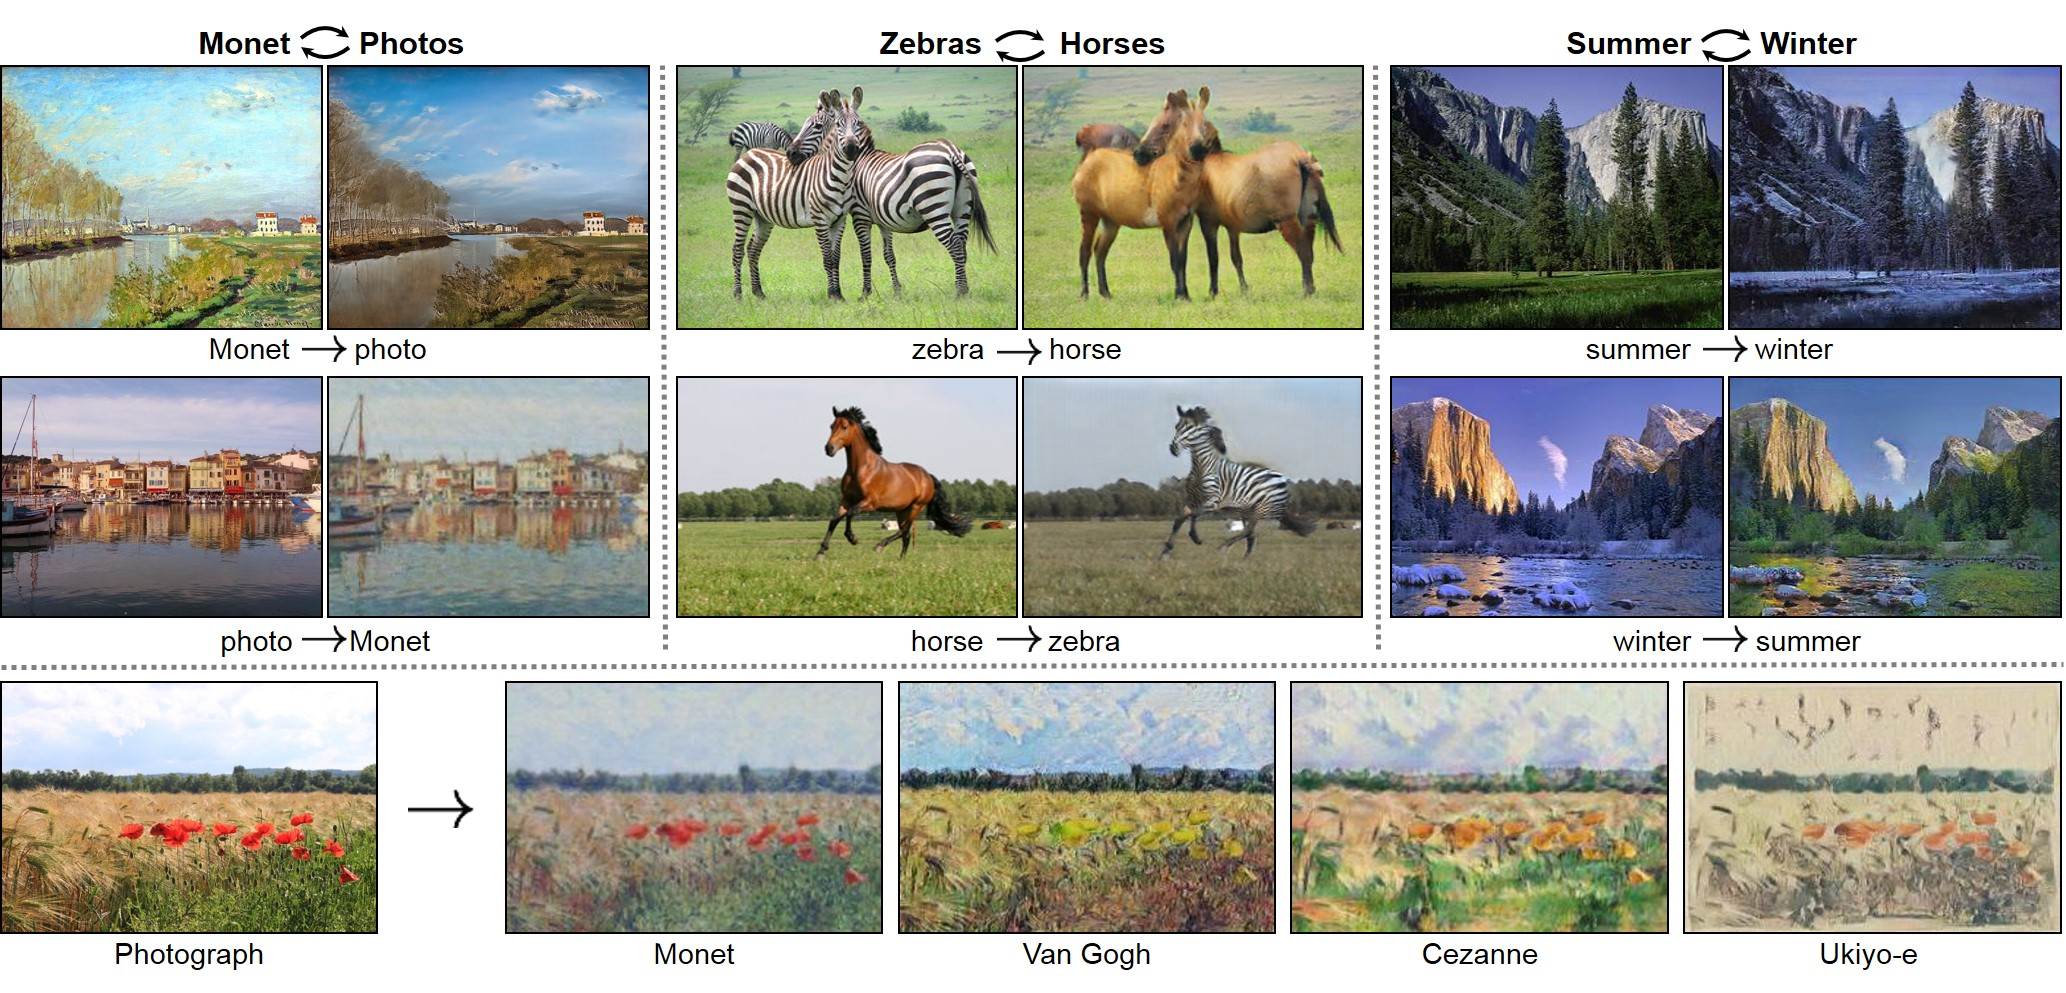
\includegraphics[scale=0.4]{img/gan_img.jpg}
    \end{center}
    \caption{Figure dans le texte~\cite{CycleGAN2017}}
    \label{fig:gan}
\end{figure}

\newpage
\appendix

\section{TUTORIEL POUR L'ANNEXE}\label{appendix:fastbook}

\begin{figure}[h!]
    \begin{center}
        
\includegraphics[scale=1.3]{img/fastbook.png}
    \end{center}
    \caption{\cite{howard2020deep}}
    \label{fig:fastbook}
\end{figure}


\newpage
\bibliographystyle{IEEEtran}
% « La bibliographie est la seule chose que vous pouvez structurer en anglais
% notamment les références IEEE qui ont une rigueur stricte. » (Adjoint à la
% coordination des stages)
\bibliography{references}

\end{document}